\chapter{Projekt aplikacji}
\thispagestyle{chapterBeginStyle}
\label{rozdzial2}
W tym rozdziale przedstawiono szczegółowy projekt systemu korzystając z notacji UML oraz uwzględniając założenia funkcjonalne z rozdziału \ref{wstep}.
Scharakteryzowano przypadki użycia oraz towarzyszące im scenariusze. Przedstawiono ogólną strukturę aplikacji w diagramie komponentów. Określono tryby działania aplikacji poprzez diagram stanów. Przedstawiono projekt bazy danych. Opisano dokładnie protokół komunikacji z MiBandem 3. 

\section{Przypadki użycia}
Poniżej przedstawiono ogólny diagram przypadków użycia \ref{use_case}. Szczegółowe scenariusze zostały zdefiniowane w odpowiednich podsekcjach tego podrozdziału.
\begin{figure}[H]
    \begin{center}
        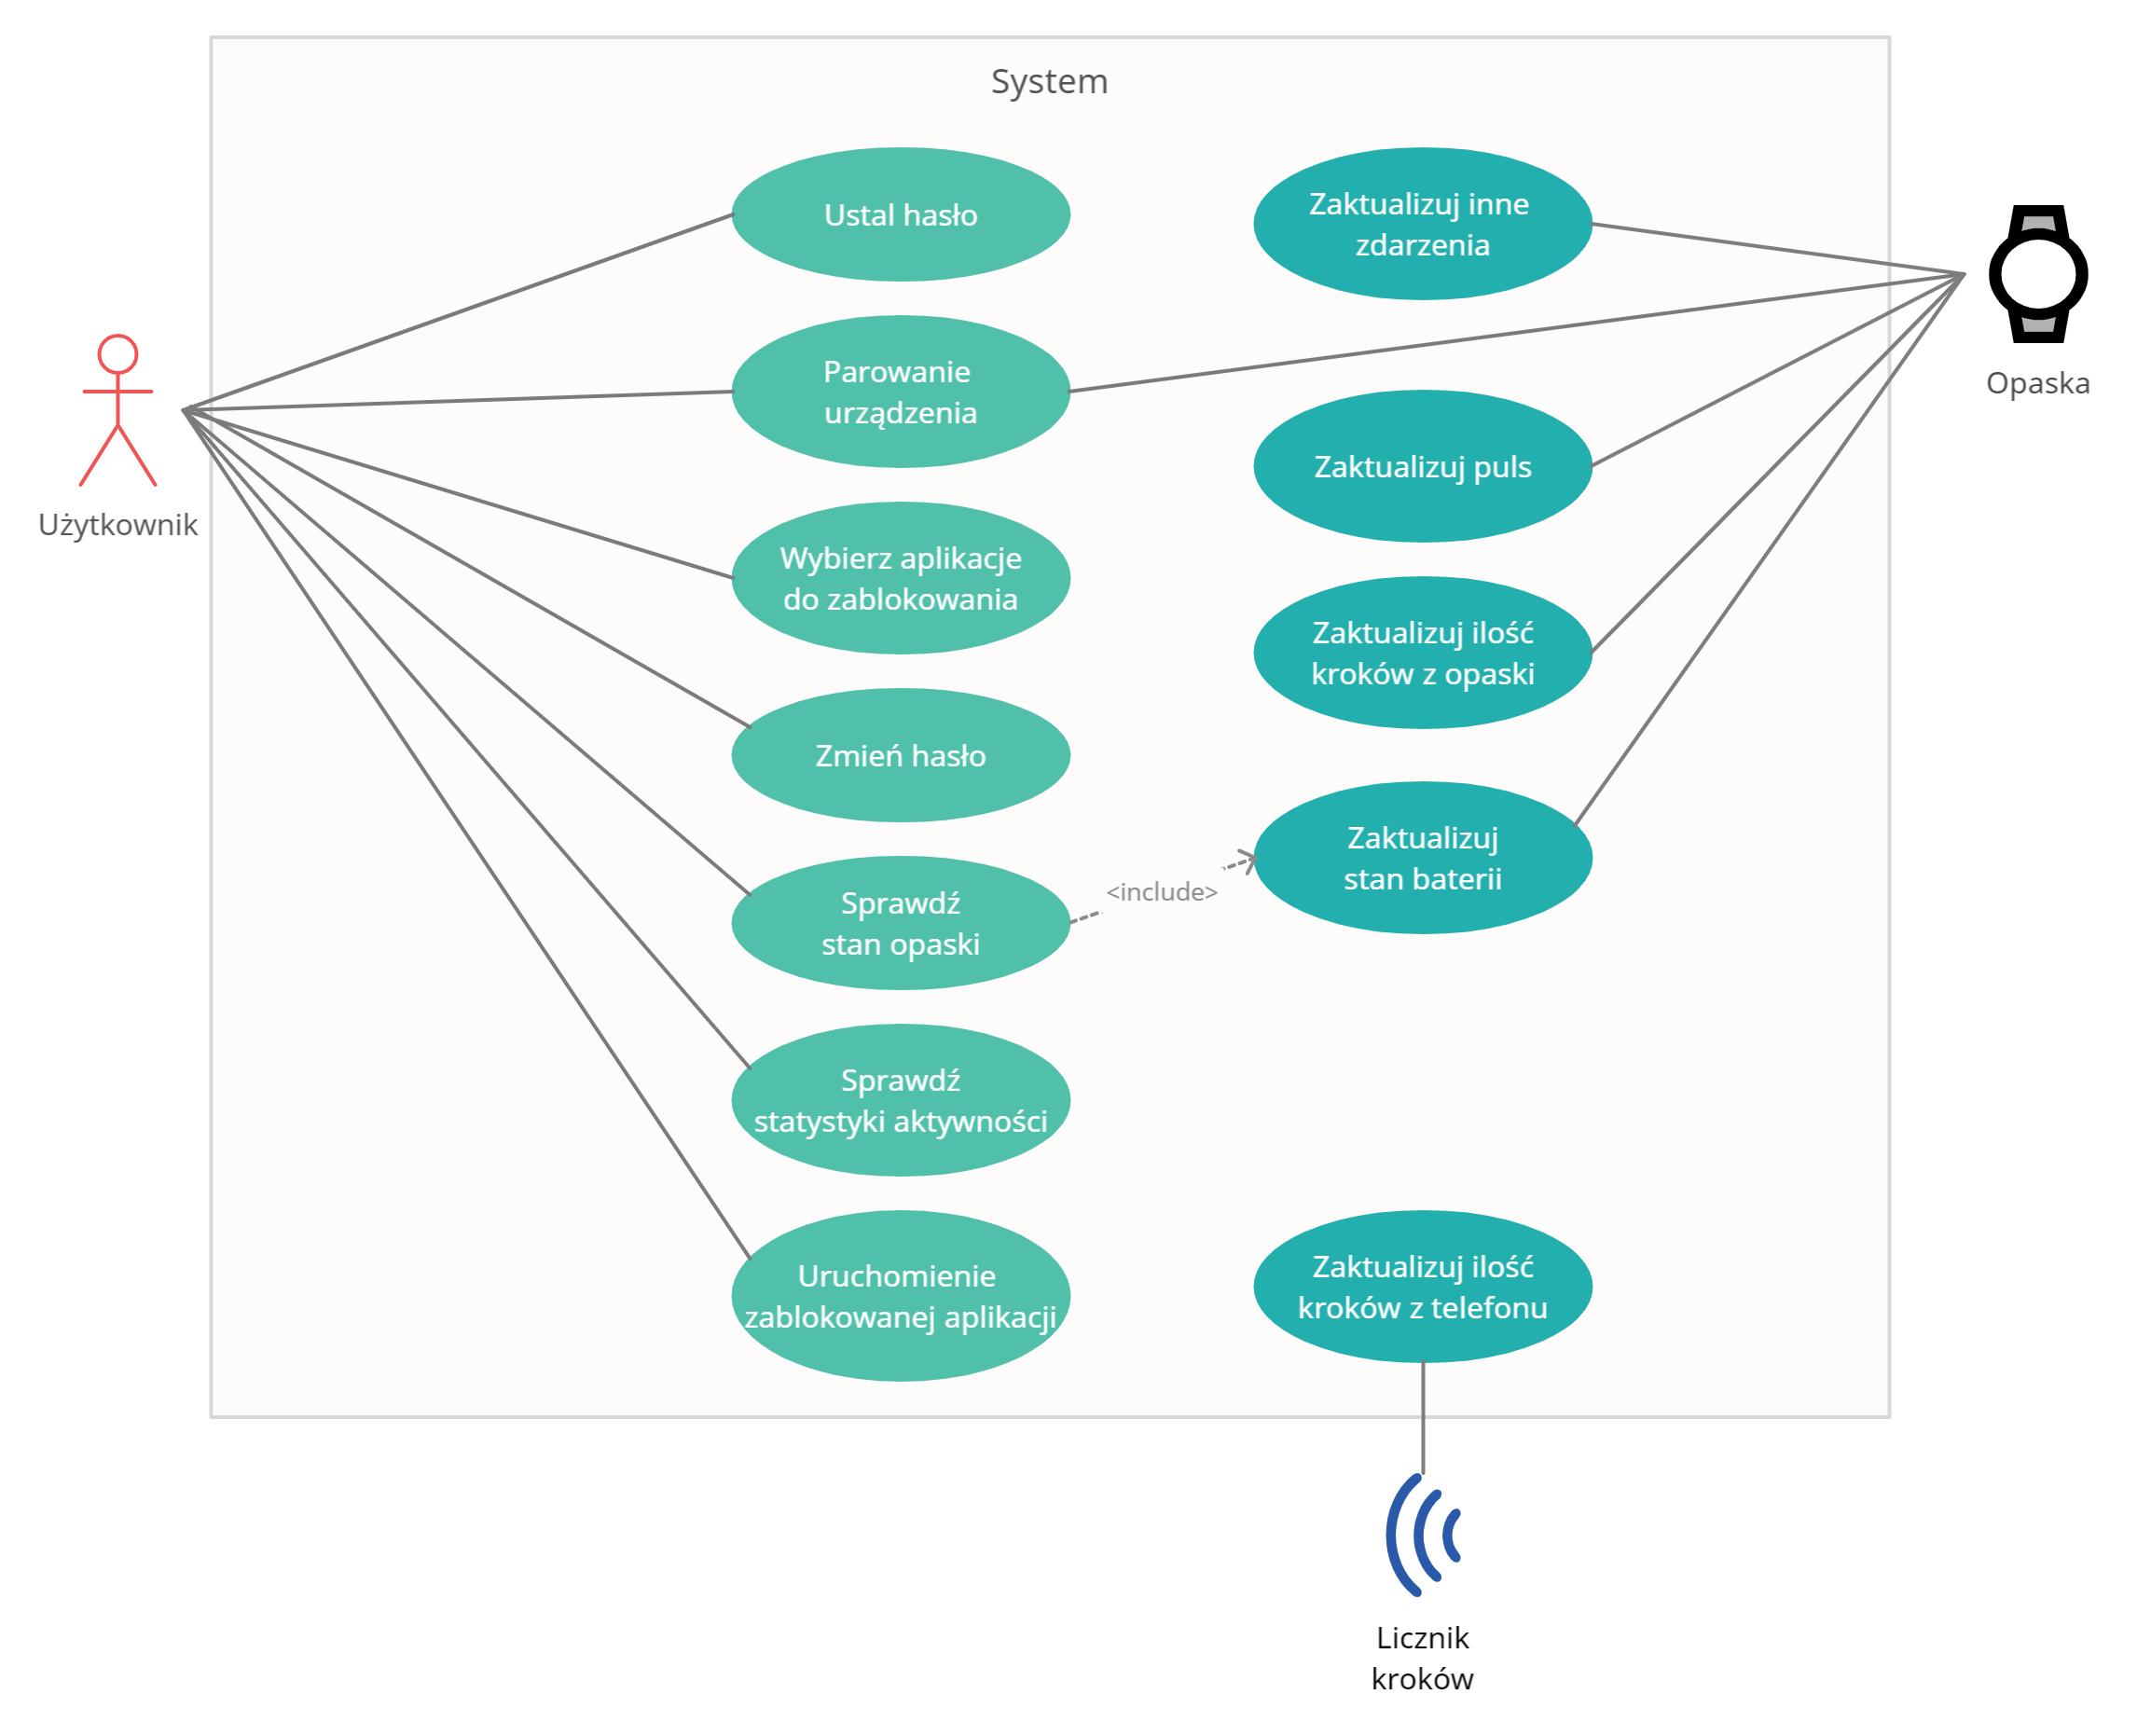
\includegraphics[width=0.9\textwidth]{UseCaseDiagram.png}
    \end{center}
    \caption{{\color{dgray}Diagram przypadków użycia w systemie.}} \label{use_case}
\end{figure}

\subsection{Ustal hasło}
W tym przypadku użytkownik aplikacji ustala hasło, które jest potrzebne przy odblokowywaniu dostępu do zablokowanych aplikacji. Aktorami są Użytkownik oraz System. Obecny przypadek użycia jest inicjowany przy pierwszym uruchomieniu aplikacji, kiedy nie istnieje jeszcze zaszyfrowany plik, w którym będzie przechowywane hasło. Po wykonaniu przypadku w systemie zostaje zarejestrowane hasło użytkownika, które będzie później wykorzystane w celu dezaktywacji blokady aplikacji. Scenariusz składa się z następującego przepływu głównego:
\begin{enumerate}
    \item Aplikacja wyświetla formularz zawierający pola Hasło oraz Powtórz hasło.
    \item Użytkownik wprowadza identyczne hasła do podanych pól oraz zatwierdza wprowadzone dane przyciskiem znajdującym się poniżej.
    \item System sprawdza zgodność haseł oraz czy spełniają wymagane kryteria.
    \item System tworzy zaszyfrowany plik i zapisuje w nim hasz hasła.
\end{enumerate}
Alternatywnie:
\newline\newline
\indent 3. Jeśli wprowadzone hasła nie są zgodne:
\begin{enumerate}[leftmargin=3\parindent]
    \item Zostaje wyświetlony komunikat o błędzie.
    \item Następuje powrót do kroku numer 2 w głównym przepływie.
\end{enumerate}

\subsection{Parowanie urządzenia}
W tym przypadku użytkownik aplikacji skanuje otoczenie, korzystając z modułu Bluetooth w poszukiwaniu najbliższej opaski MiBand, a następnie nawiązuje z nią pierwsze połączenie. Aktorami są Użytkownik, System oraz Opaska. Przypadek ten występuje przy pierwszym uruchomieniu systemu, kiedy zostało już ustalone hasło odblokowujące. Po zakończeniu system jest sparowany z opaską MiBand, z którą komunikacja jest kluczowym punktem działania systemu. W systemie zostaje także zapisany adres MAC opaski, dzięki czemu będzie można z łatwością ponownie połączyć się z nią. Główny przepływ składa się z następujących kroków:
\begin{enumerate}
    \item Użytkownik naciska przycisk ``Skan''.
    \item System rozpoczyna skanowanie urządzeń Bluetooth Low Energy w celu znalezienia Opaski.
    \item System wyświetla znalezione Opaski w formie listy. 
    \item Użytkownik wybiera Opaskę, do której się podłączy poprzez naciśnięcie na jej nazwę.
    \item System tworzy więź z wybraną Opaską i inicjuje pierwsze połączenie.
\end{enumerate}
Alternatywnie:
\newline\newline
\indent 3. Jeśli nie znaleziono żadnej Opaski:
\begin{enumerate}[leftmargin=3\parindent]
    \item Zostaje wyświetlony komunikat o błędzie.
    \item Następuje powrót do kroku numer 1 w głównym przepływie.
\end{enumerate}
\quad\newline
\indent 5. Jeśli wystąpi błąd połączenia z Opaską:
\begin{enumerate}[leftmargin=3\parindent]
    \item Następuje powrót do kroku numer 4 w głównym przepływie.
\end{enumerate}

\subsection{Wybierz aplikacje do zablokowania}
W tym przypadku użytkownik aplikacji wybiera z listy zainstalowanych aplikacji te, które będą blokowane przez system kiedy zostanie uruchomiona blokada. Aktorami są Użytkownik oraz System. Przypadek ten występuje, gdy istnieje plik z hasłem, opaska została sparowana, nie ma uruchomionej blokady oraz Użytkownik uruchomił aplikację. Po zakończeniu System posiada informację, na których aplikacjach uruchamiać blokadę. Główny przepływ składa się z następujących kroków:
\begin{enumerate}
    \item Użytkownik z poziomu głównego ekranu aplikacji przechodzi do Ustawień.
    \item Użytkownik wybiera opcję Zablokowane aplikacje.
    \item Użytkownik zaznacza aplikację z listy, którą chce zablokować bądź odblokować.
    \item System zapisuje aktualny stan aplikacji.
\end{enumerate}

\subsection{Zmień hasło}
W tym przypadku użytkownik aplikacji zmienia hasło odblokowujące dostęp do zablokowanych aplikacji. Aktorami są Użytkownik oraz System. Przypadek ten występuje, gdy istnieje plik z hasłem, opaska została sparowana, nie ma uruchomionej blokady oraz Użytkownik uruchomił aplikację. Po zakończeniu System posiada informację o nowym haśle, które będzie wykorzystywane od tej pory do odblokowywania dostępu. Główny przepływ składa się z następujących kroków:
\begin{enumerate}
    \item Użytkownik z poziomu głównego ekranu aplikacji wybiera opcję Ustawienia w dolnej nawigacji.
    \item Użytkownik wybiera opcję Zmień hasło.
    \item Użytkownik wpisuje odpowiednie wartości do pól Stare hasło, Nowe hasło oraz Powtórz nowe hasło oraz zatwierdza wprowadzone dane.
    \item System zapisuje hasz nowego hasła w zaszyfrowanym pliku.
\end{enumerate}
Alternatywnie: 
\newline\newline
\indent 3. Jeśli stare hasło jest błędne lub nowe hasło nie zgadza się z powtórzonym:
\begin{enumerate}[leftmargin=3\parindent]
    \item System wyświetla komunikat o błędnych wprowadzonych danych.
    \item Następuje powrót do kroku numer 3 w głównym przepływie.
\end{enumerate}
\quad\newline
\indent 4. Jeśli wystąpi błąd zapisu:
\begin{enumerate}[leftmargin=3\parindent]
    \item System wyświetla komunikat o błędzie zapisu.
    \item Następuje powrót do kroku numer 3 w głównym przepływie.
\end{enumerate}

\subsection{Sprawdź stan opaski}
W tym przypadku użytkownik aplikacji sprawdza podstawowe informacje na temat opaski oraz jej stan baterii. Aktorami są Użytkownik, System oraz Opaska. Przypadek ten występuje, gdy istnieje plik z hasłem, opaska została sparowana, nie ma uruchomionej blokady oraz Użytkownik uruchomił aplikację. Po zakończeniu Użytkownik zna stan baterii oraz inne informacje o Opasce, a System zyskuje odświeżony stan baterii Opaski. Głowny przepływ składa się z następujących kroków:
\begin{enumerate}
    \item Użytkownik z poziomu głównego ekranu aplikacji wybiera opcję Opaska w dolnej nawigacji.
    \item System wyświetla zapisane wcześniej informacje o Opasce.
    \item Przejdź do przypadku Zaktualizuj stan baterii
    \item System aktualizuje wartość baterii na ekranie.
\end{enumerate}
Alternatywnie:
\newline\newline
\indent 2. Jeśli nie zapisano wcześniej informacji o Opasce:
\begin{enumerate}[leftmargin=3\parindent]
    \item System wyświetla w brakujących polach wartość Nieznane.
    \item Następuje przejście do kroku numer 3 w głównym przepływie.
\end{enumerate}
\quad\newline
\indent 3. Jeśli nastąpi nagła utrata połączenia z Opaską:
\begin{enumerate}[leftmargin=3\parindent]
    \item Pomiń następny krok w głównym przepływie.
\end{enumerate}

\subsection{Sprawdź statystyki aktywności}
W tym przypadku użytkownik aplikacji sprawdza proste statystyki zarejestrowanej dziennej aktywności. Aktorami są Użytkownik oraz System. Przypadek ten występuje, gdy istnieje plik z hasłem, opaska została sparowana, nie ma uruchomionej blokady oraz Użytkownik uruchomił aplikację. Po zakończeniu Użytkownik zna ilość zarejestrowanych kroków oraz ostatnią zarejestrowaną wartość pulsu. Główny przepływ składa się z następujących kroków:
\begin{enumerate}
    \item Użytkownik z poziomu głównego ekranu aplikacji wybiera opcję Statystyki w dolnej nawigacji.
    \item System wyświetla ostatnie zapisane wartości dziennych kroków oraz pulsu.
    \item System aktualizuje wyświetlane wartości, gdy zostaną zapisane nowe.
\end{enumerate}

\subsection{Uruchomienie zablokowanej aplikacji}
W tym przypadku użytkownik aplikacji próbuje uruchomić aplikację z listy zablokowanych podczas, gdy uruchomiona jest blokada. Aktorami są Użytkownik i System. Przypadek ten występuje, gdy istnieje plik z hasłem, opaska została sparowana oraz aplikacja pracuje w trybie blokady. Po zakończeniu Użytkownik posiada autoryzację do interakcji z blokowanymi aplikacjami, a System przechodzi w tryb monitorowania. Główny przepływ składa się z następujących kroków:
\begin{enumerate}
    \item Użytkownik uruchamia aplikację z listy zablokowanych.
    \item System przenosi Użytkownika w ekran wprowadzania hasła.
    \item Użytkownik wprowadza hasło i zatwierdza.
    \item System wyłącza blokadę i uruchamia usługę monitorującą.
\end{enumerate}
Alternatywnie:
\newline\newline
\indent 3. Jeśli Użytkownik wprowadził błędne hasło:
\begin{enumerate}[leftmargin=3\parindent]
    \item System wyświetla komunikat o błędnym haśle.
    \item Następuje ponowne wykonanie kroku 3 z głównego przepływu.
\end{enumerate}

\subsection{Zaktualizuj inne zdarzenia}
W tym przypadku opaska rejestruje jedno z podejrzanych zdarzeń i przesyła informację o tym do aplikacji. Aktorami są Opaska oraz System. Przypadek ten występuje, gdy istnieje plik z hasłem, opaska została sparowana i jest aktywne połączenie między nią a aplikacją. Po zakończeniu System zyskuje sygnał do uruchomienia blokady. Główny przepływ składa się z następujących kroków:
\begin{enumerate}
    \item Opaska rejestruje jedno z zaprogramowanych zdarzeń.
    \item Opaska przesyła kod zdarzenia do Systemu.
    \item System porównuje otrzymany kod z zapisanymi kodami podejrzanych zdarzeń.
    \item System uruchamia blokadę.
\end{enumerate}
Alternatywnie:
\newline\newline
\indent 2. Jeśli nastąpi nagła utrata połączenia:
\begin{enumerate}[leftmargin=3\parindent]
    \item Następuje przejście do kroku numer 4 w głównym przepływie.
\end{enumerate}
\quad\newline
\indent 3. Jeśli otrzymany kod nie znajduje się na liście podejrzanych:
\begin{enumerate}[leftmargin=3\parindent]
    \item Pomiń następny krok głównego przepływu.
\end{enumerate}
\subsection{Zaktualizuj puls}
W tym przypadku opaska wykonuje automatyczny pomiar pulsu i przesyła jego wartość do aplikacji. Aktorami są Opaska oraz System. Przypadek ten występuje, gdy istnieje plik z hasłem, opaska została sparowana i jest aktywne połączenie między nią a aplikacją. Po zakończeniu System zyskuje aktualne dane na temat pulsu do analizy stanu użytkownika. Główny przepływ składa się z następujących kroków:
\begin{enumerate}
    \item Opaska mierzy puls.
    \item Opaska przesyła zarejestrowaną wartość do Systemu.
    \item System zapisuje otrzymaną wartość.
\end{enumerate}
Alternatywnie:
\newline\newline
\indent 2. Jeśli nastąpi nagła utrata połączenia:
\begin{enumerate}[leftmargin=3\parindent]
    \item System uruchamia blokadę.
\end{enumerate}
\quad\newline
\indent 3. Jeśli otrzymana wartość wynosi 0:
\begin{enumerate}[leftmargin=3\parindent]
    \item System uruchamia blokadę.
\end{enumerate}

\subsection{Zaktualizuj ilość kroków z opaski}
W tym przypadku opaska rejestruje wykonane kroki oraz przesyła uaktualnioną wartość dziennych wykonanych kroków do aplikacji. Aktorami są Opaska oraz System. Przypadek ten występuje, gdy istnieje plik z hasłem, opaska została sparowana i jest aktywne połączenie między nią a aplikacją. Po zakończeniu System zyskuje aktualne dane na temat wykonanych kroków, które zostaną wykorzystane później do analizy zachowania użytkownika. Główny przepływ składa się z następujących kroków:
\begin{enumerate}
    \item Opaska rejestruje wykonanie kroków.
    \item Opaska przesyła zaktualizowaną wartość dziennych kroków do Systemu.
    \item System zapisuje otrzymaną wartość.
\end{enumerate}
Alternatywnie:
\newline\newline
\indent 2. Jeśli nastąpi nagła utrata połączenia:
\begin{enumerate}[leftmargin=3\parindent]
    \item System uruchamia blokadę.
\end{enumerate}
\quad\newline
\indent 3. Jeśli otrzymana wartość jest równa ostatniemu pomiarowi:
\begin{enumerate}[leftmargin=3\parindent]
    \item System nie zapisuje otrzymanej wartości.
\end{enumerate}

\subsection{Zaktualizuj stan baterii}
W tym przypadku aplikacja odczytuje aktualny stan baterii z opaski. Aktorami są Opaska oraz System. Przypadek ten występuje, gdy istnieje plik z hasłem, opaska została sparowana i jest aktywne połączenie między nią a aplikacją. Po zakończeniu System zyskuje aktualną wartość stanu baterii. Główny przepływ składa się z następujących kroków:
\begin{enumerate}
    \item System przesyła do Opaski zapytanie o stan baterii.
    \item Opaska przesyła do Systemu aktualny stan baterii.
    \item System zapisuje nową wartość stanu baterii.
\end{enumerate}
Alternatywnie:
\newline\newline
\indent 2. Jeśli nastąpi nagła utrata połączenia:
\begin{enumerate}[leftmargin=3\parindent]
    \item System uruchamia blokadę.
\end{enumerate}

\subsection{Zaktualizuj ilość kroków z telefonu}
W tym przypadku sensor licznika kroków w smartfonie rejestruje wykonane kroki, a następnie informuje aplikację o aktualizacji swojej wartości. Aktorami są Licznik kroków oraz System. Przypadek ten występuje, gdy istnieje plik z hasłem, opaska została sparowana i jest aktywna usługa monitorująca zachowanie użytkownika. Po zakończeniu System zyskuje informację na temat wykonanych kroków, która zostanie później wykorzystana do analizy zachowania użytkownika.
\begin{enumerate}
    \item Licznik kroków rejestruje wykonanie kroków.
    \item System odczytuje zaktualizowaną liczbę kroków Licznika kroków.
    \item System zapisuje odczytaną wartość.
\end{enumerate}

\section{Diagram komponentów}

W tej sekcji należy przedstawić diagramy komponentów dla odpowiednich elementów systemu zidentyfikowane na podstawie wcześniejszych rozważań

\section{Diagramy stanów}

W tej sekcji należy przedstawić diagramy stanów w których może znaleźć się system. Diagramy te są szczególnie istotne przy projektowaniu systemów czasu rzeczywistego.

\section{Projekt bazy danych}

W tej sekcji należy przedstawić projekt bazy danych. Należy omówić wycinek rzeczywistości i odpowiadające mu zidentyfikowane elementy systemu, których wartości będą podlegać utrwalaniu. Należy przedyskutować wybór typów danych dla atrybutów poszczególnych obiektów.  

\section{Komunikacja z MiBand 3}
W projektowanym systemie główną rolę gra inteligentna opaska. Komunikuje się ona ze smartfonem przy użyciu Bluetooth Low Energy protokołem ATT korzystając z GATT. BLE w porównaniu do klasycznego połączenia Bluetooth wykorzystuje znacznie niższe zasoby energii zachowując podobny zasięg, dzięki czemu znalazło szerokie zastosowanie w urządzeniach peryferyjnych. W poniższych podrozdziałach opisano pokrótce pojęcia ATT i GATT oraz dokładnie przedstawiono zaimplementowany protokół komunikacji z opaską MiBand 3.
\subsection{ATT}
Protokół Attribute umożliwia urządzeniu, określonemu jako \textit{serwer}, odsłonić zbiór atrybutów i powiązanych z nimi wartości urządzeniu równorzędnemu, określonemu jako \textit{klient}. Atrybuty odsłonięte przez serwer mogą być odkryte, odczytane bądź nadpisane przez klienta, a także mogą być rozgłaszane przez serwer w ramach powiadomienia lub zasygnalizowania. Atrybut jest dyskretną wartością o trzech właściwościach powiązanych ze sobą:
\begin{itemize}
    \item typie,
    \item uchwycie,
    \item zestawie pozwoleń, które są zdefiniowane przez specyfikację wyższej warstwy wykorzystującą dany atrybut.
\end{itemize}
Typ atrybutu określa, co reprezentuje dany atrybut poprzez UUID (Universally Unique Identifier), ktore może zostać utworzone przez każdego, a następnie zostać opublikowane. Pozwala to rozpoznać atrybut niezależnie od nadanego mu przez serwer uchwytu. Uchwyt atrybutu jest unikalną, niezerową, 16-bitową wartością, która jednoznacznie identyfikuje dany atrybut w obrębie serwera, pozwalając klientowi odnieść się do niego podczas operacji odczytu oraz zapisu. Pozwolenia mogą być nadane atrybutowi w celu ograniczenia klientowi dostępu do zapisu lub odczytu.
\newline\newline
\indent Urządzenie może jednocześnie implementować zarówno rolę serwera jak i klienta oraz obie role mogą funkcjonować współbieżnie oraz komunikować się między sobą. Na każdym urządzeniu Bluetooth może znajdować się maksymalnie jedna instancja serwera.
\newline\newline
\indent Wszystkie prośby protokołu Attribute są przesyłane poprzez \textit{nosiciela ATT}. Między urządzeniami może być wielu nosicieli, gdzie każdy z nich korzysta z osobnego kanału L2CAP oraz może mieć inną konfigurację. W przypadku BLE, wykorzystywany jest pojedynczy nosiciel ATT, który używa stałego kanału dostępnego od ustanowienia połączenia ACL. Można jednak skonfigurować dodatkowych nosicieli używając L2CAP. Więcej informacji na temat protokołu ATT można znaleźć w \cite{BT-Corev5.2}. 

\subsection{GATT}
Profil Generic Attribute (GATT) definiuje framework wykorzystujący protokół Attribute, określający procedury i formaty danych znajdujących się wewnątrz profilu. Zdefiniowane procedury obejmują odkrywanie, odczyt, zapis, powiadamianie oraz sygnalizację. Profil ten został zaprojektowany do wykorzystania przez aplikacje bądź inny profil, aby umożliwić klientowi komunikację z serwerem poprzez opakowanie protokołu ATT w bardziej przystępną formę.
\newline\newline
\indent Profil GATT określa strukturę, w której odbywa się wymiana danych. Najwyższym poziomem jest profil zawierający liczne \textit{usługi} będące zbiorem danych oraz przypisanych im zachowań niezbędnych do zapewnienia określonej funkcji. Usługi składają się z \textit{charakterystyk}, z których każda zawiera określoną wartość oraz opcjonalne informacje na jej temat. Usługi oraz charakterystyki wraz ze swoimi komponentami zawierają dane profilu, które są przechowywane w Atrybutach na serwerze. Dzięki wykorzystaniu określonej struktury danych przez GATT możliwe jest przeglądanie dostępnych Usług oraz Charakterystyk, nawet gdy klient nie jest wyspecjalizowany pod dany serwer. Więcej informacji na temat GATT można znaleźć w \cite{BT-Corev5.2}.

\subsection{Wykorzystane usługi i charakterystyki}
Do uzyskania potrzebnych danych z opaski zostały użyte poniżej opisane usługi. Dla każdej z nich przedstawiono listę wykorzystanych charakterystyk z krótkim opisem, za co odpowiadają. Poniższe wartości zostały zidentyfikowane na podstawie przechwytywania pakietów ATT komunikacji MiBanda 3 z aplikacją Gadgetbridge \cite{Gadgetbridge} przy użyciu open-sourcowego sniffera Wireshark \cite{Wireshark} oraz analizie kodu źródłowego Gadgetbridge.

\subsubsection{0000fee0-0000-1000-8000-00805f9b34fb}
Jest to usługa odpowiadająca w głównej mierze za podstawowe funkcjonalności opaski MiBand 3. Pozwala zmodyfikować ustawienia urządzenia, zapisać informacje o użytkowniku oraz odczytać dane o stanie baterii i aktywności użytkownika. Jest to najczęściej wykorzystywana usługa w aplikacji.

\begin{table}[H]
    \bgroup
    \def\arraystretch{1.5}%
    \begin{tabular}{|ll|}
    \hline
    \textbf{Charakterystyka}                      & \textbf{Opis}                                                                                                                \\ \hline
    \textbf{00000003-0000-3512-2118-0009af100700} & \begin{tabular}[c]{@{}l@{}}Charakterystyka pozwalająca na konfigurację ustawień \\ opaski.\end{tabular}                      \\
    \textbf{00000006-0000-3512-2118-0009af100700} & \begin{tabular}[c]{@{}l@{}}Charakterystyka zawierająca informacje o stanie baterii \\ opaski.\end{tabular}                   \\
    \textbf{00000007-0000-3512-2118-0009af100700} & \begin{tabular}[c]{@{}l@{}}Charakterystyka przechowująca liczbę wykonanych kroków \\ danego dnia.\end{tabular}               \\
    \textbf{00000008-0000-3512-2118-0009af100700} & Charakterystyka zawierająca dane użytkownika.                                                                                \\
    \textbf{00000010-0000-3512-2118-0009af100700} & \begin{tabular}[c]{@{}l@{}}Charakterystyka zawierająca informacje na temat zdarzeń \\ wykrywanych przez opaskę.\end{tabular} \\
    \textbf{00002a2b-0000-1000-8000-00805f9b34fb} & Charakterystyka przechowująca aktualną datę i godzinę,                                                                       \\ \hline
    \end{tabular}
    \egroup
    \caption{{\color{dgray}Wykorzystane charakterystyki z usługi 0000fee0-0000-1000-8000-00805f9b34fb.}} \label{miliservice}
\end{table}

\subsubsection{0000fee1-0000-1000-8000-00805f9b34fb}
Jest to usługa zawierająca przede wszystkim charakterystykę wykorzystywaną w procesie autentykacji połączenia oraz parowania. W usłudze tej znajduje się też sporo niezidentyfikowanych charakterystyk, które nie są wymagane do działania aplikacji. Dlatego więc zostały pominięte.
\begin{table}[H]
    \bgroup
    \def\arraystretch{1.5}%
    \begin{tabular}{|ll|}
    \hline
    \textbf{Charakterystyka}                      & \textbf{Opis}                                                                                                                \\ \hline
    \textbf{00000009-0000-3512-2118-0009af100700} & \begin{tabular}[c]{@{}l@{}}Charakterystyka wykorzystywana do autentykacji  \\ połączenia między opaską a klientem\end{tabular} \\ \hline
    \end{tabular}
    \egroup
    \caption{{\color{dgray}Wykorzystane charakterystyki z usługi 0000fee1-0000-1000-8000-00805f9b34fb.}} \label{miband2service}
\end{table}

\subsubsection{0000180d-0000-1000-8000-00805f9b34fb}
Jest to usługa zdefiniowana przez Bluetooth Special Interest Group odpowiadająca za komunikację między sensorem akcji serca a innym klientem GATT. Za jej pomocą można uzyskać informację o pulsie użytkownika oraz skonfigurować automatyczne pomiary. 

\begin{table}[H]
    \bgroup
    \def\arraystretch{1.5}%
    \begin{tabular}{|ll|}
    \hline
    \textbf{Charakterystyka}                      & \textbf{Opis}                                                                                                              \\ \hline
    \textbf{00002a37-0000-1000-8000-00805f9b34fb} & \begin{tabular}[c]{@{}l@{}}Charakterystyka wykorzystywana do odczytu aktualnej \\ wartości pulsu użytkownika.\end{tabular} \\
    \textbf{00002a39-0000-1000-8000-00805f9b34fb} & \begin{tabular}[c]{@{}l@{}}Charakterystyka odpowiedzialna za konfigurację sensora \\ akcji serca w opasce.\end{tabular}    \\ \hline
    \end{tabular}
    \egroup
    \caption{{\color{dgray}Wykorzystane charakterystyki z usługi 0000180d-0000-1000-8000-00805f9b34fb.}} \label{heartrateservice}
\end{table}

\subsubsection{0000180a-0000-1000-8000-00805f9b34fb}
Jest to usługa również zdefiniowana przez Bluetooth Special Interest Group. Odpowiada za dostarczenie informacji o urządzeniu. W tym wypadku jest to informacja o numerze seryjnym opaski oraz wersjach sprzętu i oprogramowania.

\begin{table}[H]
    \bgroup
    \def\arraystretch{1.5}%
    \begin{tabular}{|ll|}
    \hline
    \textbf{Charakterystyka}                      & \textbf{Opis}                                                                                                      \\ \hline
    \textbf{00002a25-0000-1000-8000-00805f9b34fb} & \begin{tabular}[c]{@{}l@{}}Charakterystyka wykorzystywana do odczytu numeru \\ seryjnego opaski.\end{tabular}      \\
    \textbf{00002a27-0000-1000-8000-00805f9b34fb} & \begin{tabular}[c]{@{}l@{}}Charakterystyka wykorzystywana do odczytu wersji \\ sprzętu opaski.\end{tabular}        \\
    \textbf{00002a28-0000-1000-8000-00805f9b34fb} & \begin{tabular}[c]{@{}l@{}}Charakterystyka wykorzystywana do odczytu wersji \\ oprogramowania opaski.\end{tabular} \\ \hline
    \end{tabular}
    \egroup
    \caption{{\color{dgray}Wykorzystane charakterystyki z usługi 0000180a-0000-1000-8000-00805f9b34fb.}} \label{deviceservice}
\end{table}

\subsection{Autentykacja połączenia}
\subsection{Sekwencja startowa}
\subsection{Inne operacje}
